\subsection{Total Variation(TV) Based Applications}
\label{subsec:TV Applications}

%Total variation(TV) For a function$f(x)$ defined on a domain $\Omega\subseteq\mathbb{R}^n$, its TV is defined as
%
%\small{
%\begin{equation}
% \label{eq:continuousTV1}
% J_{f}=\int_{\Omega}^{}| \nabla f |dx,
%\end{equation}
%}
%\\
%where $| \nabla f |$ is the $\ell_2$-norm of the gradient $\nabla f$, i.e.,
%
%\small{
%\begin{equation}
% \label{eq:continuousTV2}
% | \nabla f |= \sqrt{ \sum_{i=1}^{} ( \frac{\partial f} {\partial x_{i}} )^2}.
%\end{equation}
%}
%\\

Total variation(TV) has been a popular tool for image processing tasks,
such as denoising, reconstruction, and segmentation\cite{chambolle2010introduction},
the underlying model for TV methods aims at exploiting the sparsity of the gradient of the image.
The discrete variant yields the following convex objective function

\small{
\begin{equation}
 \label{eq:descreteTV}
 TV(u)=\sum_{i,j}^{}\|\mathcal{D}_{i,j}u\|_2
\end{equation}
}
\\
where $\mathcal{D}_{i,j}$ is the discrete gradient operator at pixel $(i,j)$ and $u$ is a vector containing the gray-level pixel values. TV methods filter the image by minimizing $TV(u)$ which is in fact the $\ell_1$ norm of the vector $[\cdots~\|\mathcal{D}_{i,j}u\|_2~\cdots]$.

Since TV is designed for images, it is not directly applicable to geometry processing problem.
As we have stated, the key point is to find some form of second order information.


\subsubsection{Point cloud consolidation}
\label{subsubsec:TVPoint cloud consolidation}

In section~\ref{subsec:Point Cloud Consolidation}, there have been several consolidation works based on $\ell_1$ median.
Here we introduce one more well-known work.
Similar to the sparse gradient minimization, and based on the observation that the gradients(normal differences) of smooth surface normals(normal differences) are sparse,
\cite{avron2010L1} formulates the piecewise smoothness reconstruction problem as a sparse minimization of orientation differences and position projections as following

\small{
\begin{equation}
 \label{eq:TVconsolidation1}
 \begin{aligned}
 &N^{out} =\mathop{\argmin}_{N} \sum_{(p_{i},p_{j})\in E}^{} w_{i,j}\|n_{i}-n_{j}\|_2\\
 &\mathrm{s.t.}~\forall i~\|n_{i}-{n_{i}}^{in}\|_2\le \gamma_{n}
 \end{aligned}
\end{equation}
}
\small{
\begin{equation}
 \label{eq:TVconsolidation2}
 X^{out} = \mathop{\argmin}_{X} \sum_{(p_{i},p_{j})\in E}^{} w_{i,j}|n_{i,j}\cdot (x_{i}-x_{j})|
\end{equation}
}
\\
where $\{n_{i}\}$ denote the surface normals, $\{x_{i}\}$ denote the point positions and $\{w_{i,j}\}$ is a set of the weight whose role is to achieve lower-than-$\ell_1$ sparsity.

Convexity of these two problems allows for finding a global optimum and deriving efficient solvers.
Figure~\ref{fig:TV consolidation} shows a well reconstructed example with sharp features.
Due to the global nature, this algorithm is extremely slow.
And it may fail for the point set with severe noises and outliers.

\begin{figure}[ht]
  \centering
  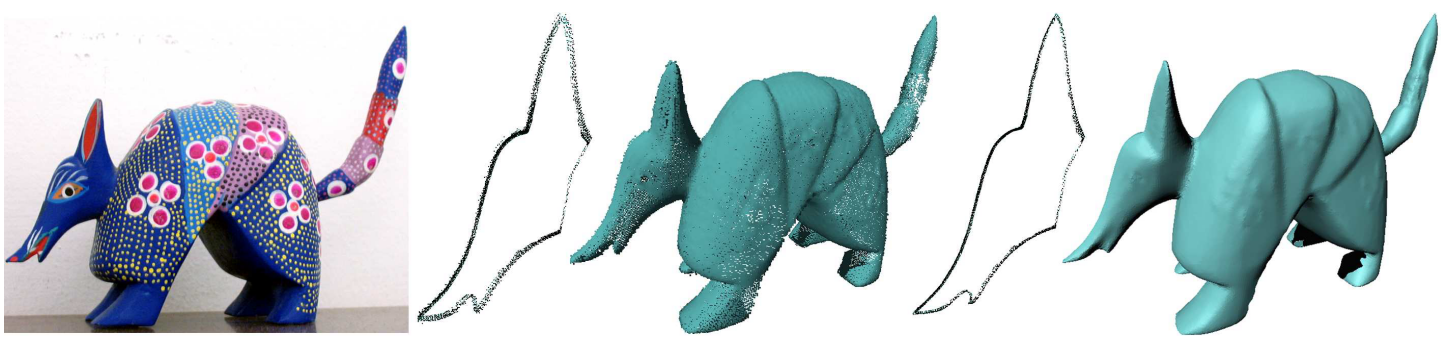
\includegraphics[width=3in]{images/TV_consolidation}
  \caption{Sparse regularization: TV based point cloud consolidation\cite{lipman2007parameterization}. The Armadillo statue(left) is scanned generating a noisy point-cloud(middle). The right figure shows the consolidation result preserving the sharp features.}
  \label{fig:TV consolidation}
\end{figure}


\subsubsection{Decomposition}
\label{subsubsection:Decompsition}

Mesh decomposition aims at segmenting a mesh into meaningful parts which are consistent with user intention, geometric mesh attributes, and human shape perception.
Generally, the elements within the same segment should have high similarity, the segment boundary should be tight and smooth as well as matching human perception, and obviously the segmentation should reflect significant features.

Motivated by the preceding observation, \cite{zhang2012variational} proposes a new method based on the Mumford-Shah model(M-S model)\cite{mumford1989optimal} that has proven successful in image segmentation, i.e., this method is also an extension from 2D images to 3D meshes.

In 2D image $I:\Omega\rightarrow \mathbb{R}^2$, the Mumford-Shah image segmentation is to find a partition $\Omega=\bigcup{_{i=1}^{k}}\Omega_{i}$, where $\Omega_{i}$ are pairwise disjoint, and numbers $c_{i}$ for $\Omega_{i}$ formulated as

\small{
\begin{equation}
 \label{eq:TV image M-S}
 \inf_{\Omega_{i},c_{i}} \sum_{}^{k}
 ( \int_{\Omega_{i}}^{} (I(x)-c_{i})^2dx + \frac{\mu}{2} | \partial\Omega_{i} | ),
\end{equation}
}
\\
where $\mu$ is a constant, $\partial \Omega$ and $|\partial \Omega|$ represent the boundary and the boundary length of segment $\Omega$, respectively.
The first data term measures the consistency of each segment and the second regularization term measures the boundary length.

To segment a 3D triangulated surface $M$, \cite{zhang2012variational} convexifies this difficult nonconvex problem~(\ref{eq:TV image M-S}) based on TV to get a new version of M-S model

\small{
\begin{equation}
 \label{eq:TV surface M-S}
 \min_{\mathbf{u}\in K, \chi_{i}} \left \{
 \int_{M}\langle\mathbf{u}(x), \mathbf{s}(x)\rangle +
 \mu g(x)| \nabla_{M}\mathbf{u}(x) | d\sigma
 \right\},
\end{equation}
}
\\
where $K$ is the set of vector functions $\mathbf{u}=(u_1,\cdots,u_{k})^{T}:M\rightarrow \mathbb{R}^{k}$ satisfying that for all $x\in M$ and $i\in [1,\cdots,k],u_{i}(x)\geq0$ and
$\sum_{i=1}^{k}u_{i}(x)=1; \mathbf{s}(x)=(s_1(x),\cdots,s_k(x))^T$ is a $k$-dimensional vector with $s_i(x)=(\mathbf{f}(x)-\chi_{i})^{T}(\mathbf{f}(x)-\chi_{i})$ indicating
the affinity vector $\chi_{i}$ that is associated with $M_{i}$ which is a segment.
The $\mathbf{f}(x)$ is a predefined multichannel function, which is constructed with the eigenvectors of the Laplacian matrix of the dual graph of $M$, for representing some attributions of $x$ over mesh $M$ similar to the RGB function for an image.

In~(\ref{eq:TV surface M-S}), if the affinity of $x$ with segment $M_{i}$ is large, $u_{i}(x)$ will tend to be small in order to reach the minimization, thus $u_{i}(x)$ can be viewed as the probability of $x$ being assigned to segment $M_{i}$ and $\mathbf{u}(x)$ can be used as a classification function for the segmentation.

Now that the regularization term in~(\ref{eq:TV surface M-S}) is to constrain the boundary with some geometric difference information between segments, it may fail for the relative smooth models.



\begin{figure}[ht]
  \centering
  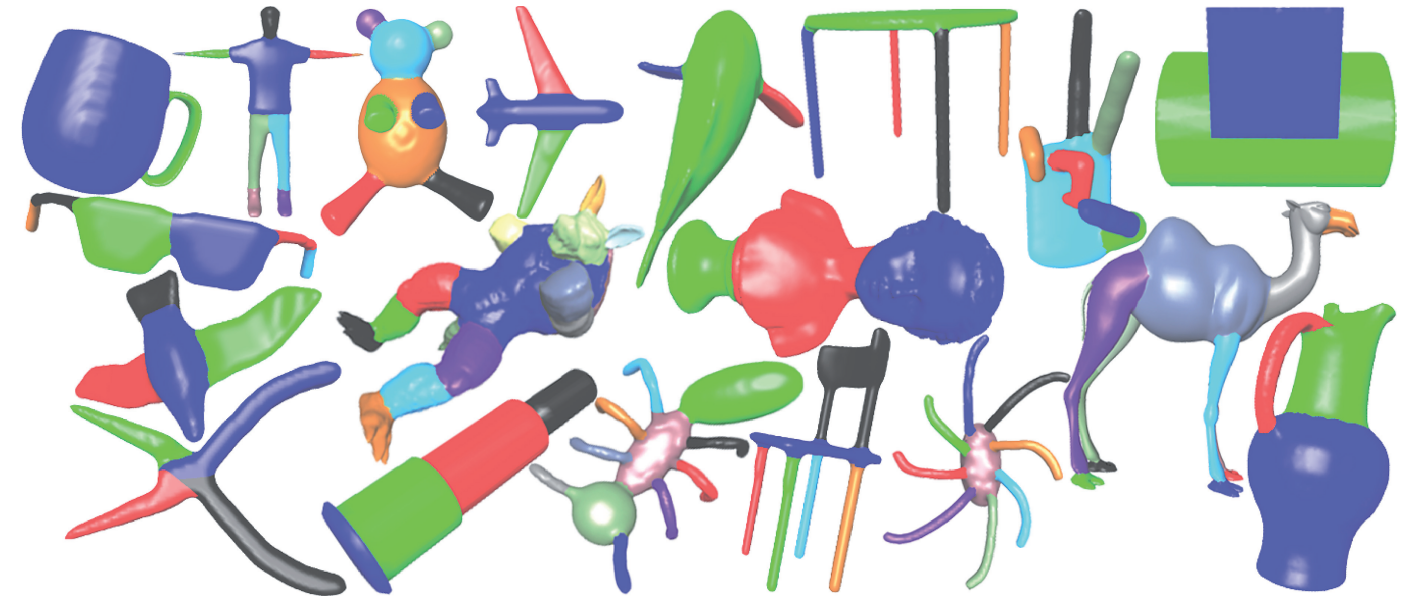
\includegraphics[width=3in]{images/segmentation}
  \caption{Sparse regularization: TV based mesh decomposition\cite{zhang2012variational}. Decomposition results where the models are taken from the Princeton Segmentation Benchmark\cite{chen2009benchmark}. One mesh is shown for each category. The segmentation results match results match human perception well in not only the cutting boundaries but also the number of segments.}
  \label{fig:segmentation}
\end{figure}


\subsubsection{Barycentric coordinates}
\label{subsubsec:Barycentric coordinates}

Barycentric~coordinates provide a simple and convenient way of interpolating values from a set of control points over the interior of a domain, using weighted combinations of values associated with different control points.

Many barycentric coordinates typically are of global nature, meaning that the interpolated value depends on many, potentially $all$, control points. Besides the lack of locality and scalability, the interpolation is computationally expensive since it involves a weighted sum of all control points for each interior vertex.
Thus, barycentric coordinates with locality provide benefit in terms of storage requirements as well as computational cost.

\cite{zhang2014local} introduces a novel method to derive $local~barycentric~coordinates$(LBC), which depend only on a small number of control points.
Given a set of control points $\mathbf{c}_1, \cdots, \mathbf{c}_n$ in $\mathbb{R}^2$ or  $\mathbb{R}^3$ which are the vertices of a closed control cage, and let the domain bounded by the cage.
They want to find a function $w_{i}$: $\Omega\rightarrow\mathbb{R}$ for each $\mathbf{c}_{i}$, such that $[w_1(\mathbf{x}), \cdots, w_n(\mathbf{x})]$ is a set of generalized barycentric coordinates of $\mathbf{x}\in\Omega$ with respect to the control points $\{\mathbf{c}_{i}\}$ and is used for interpolating function values $f(\mathbf{c}_1), \cdots, f(\mathbf{c}_n)$ at control points on the interior of $\Omega$ by

\small{
\begin{equation}
 \label{eq:BC}
 f(\mathbf{x}) = \sum_{i=1}^{n}w_{i}(\mathbf{x})f(\mathbf{c}_{i})
\end{equation}
}
\\
here, except for the properties satisfied in many barycentric coordinate schemes, like reproduction, partition of unity and non-negativity, they prefer a target functional that reflects locality and smoothness for the coordinate functions while still convex.

For a function $w_{i}$ and a given value $s$, denote by $\{w_{i}>s\}:=\{\mathbf{x}|w_{i}(\mathbf{x})>s\}$ and $\{w_{i}=s\}:=\{\mathbf{x}|w_{i}(\mathbf{x})=s\}$ the $superlevel~set$ and the $level set$ of $s$, respectively.
Locality requires the area of the superlevel set $\{w_{i}>0\}$ to be small which means that the vector$[w_{1}(\mathbf{x}), \cdots, w_{n}(\mathbf{x})]$ is sparse, while for smoothness it is necessary that all curves/surfaces $w_{i}=\textrm{const}$ are smooth.

Based on these observations, the locality and smoothness of $w_{i}$ can be obtained using a functional that measures the sum of the perimeters of superlevel sets $\{w_{i}>s\}$ for all $s$.
And then the perimeter of each superlevel set regularizes the smoothness of its boundary level curve/surface, while the perimeter of $\{w_{i}>0\}$ penalizes the area of the influence region. It turns out that this functional is exactly the total variation of $\{w_{i}\}$. Finally, the problem is formulated as

\small{
\begin{equation}
 \label{eq:continuousLBC}
 \begin{aligned}
 & \min_{w_1, \cdots, w_2} \sum_{i=1}^{n} \int_{\Omega}^{} |\bigtriangledown w_{i}| \\
 & ~~~\mathrm{s.t.}~ \sum_{i=1}^{n}w_{i}(\mathbf{x})\mathbf{c}_{i}=\mathbf{x},
        \sum_{i=1}^{n}w_{i}=1,~w_{i}\geq0,~\forall \mathbf{x}\in\Omega,\\
 & ~~~~~~~~w_{i}(\mathbf{c}_{j})=\delta_{ij},~forall i,j,\\
 & ~~~~~~~~w_{i}~\textrm{is linear on cage edges and faces }\forall i.
 \end{aligned}
\end{equation}
}
\\
Discretely, after triangulating the domain $\Omega$, each $w_{i}$ is represented a function that is linear within each cell(triangle in 2D or tetrahedron in 3D) and then the gradient of $w_{i}$ is constant on each cell. Let $\mathcal{C}$ be the set of cells in the triangulation, the target functional~\ref{eq:continuousLBC} finally becomes

\small{
\begin{equation}
 \label{eq:discreteLBC}
 \sum_{T\in\mathcal{C}}^{}  \sum_{i=1}^{}
 \phi{_{i}^{T}}  A_{T}  \| \nabla T w_{i} \|_2,
\end{equation}
}
\\
where $\nabla T w_{i}$ is the gradient of $w_{i}$ in cell $T$, $A_{T}$ is the area(volume) of $T$, and $\phi{_{i}^{T}}$ is the value of the weighting function $\phi_{i}$ at the centroid of $T$.

Figure~\ref{fig:LBC} shows a cage-based deformation example with lower computational and storage requirement since each point on the target shape is only determined by a small number of control points.
Whatever, from the observation, we can see that there is a trade-off between locality and smoothness which is a common troubling issue for so many existing works.

\begin{figure}[ht]
  \centering
  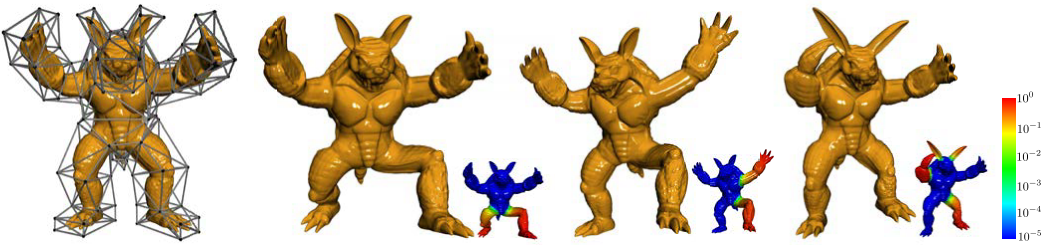
\includegraphics[width=3in]{images/LBC_L1}
  \caption{Sparse regularization: TV based local barycentric coordinates\cite{zhang2014local}. Using LBC for 3D cage-based manipulation allows for local, smooth and shape-aware deformations. Only parts near the manipulated control points are deformed, as indicated by the color-coding.}
  \label{fig:LBC}
\end{figure}
